\documentclass[a4paper,12pt]{article}
\usepackage[utf8]{inputenc}

% para separar silabas em portugues use
\usepackage[brazil]{babel}

% para indentar o primeiro parágrafo
\usepackage{indentfirst}

% para usar fontes e símbolos da AMS
\usepackage{amsfonts}
\usepackage{amssymb}
\usepackage{amsmath}

% pacotes adicionais
\usepackage{graphicx}
\usepackage{subcaption}
\usepackage{placeins}

% para ambientes do tipo theorem
\newtheorem{proposition}{\scshape Proposição}[section]
\newtheorem{corollary}{\scshape Corolário}[section]
\newtheorem{lemma}{\scshape Lema}[section]
\newtheorem{definition}{\scshape Definição}[section]
\newtheorem{conjecture}{\scshape Conjectura}[section]
\newtheorem{example}{\scshape Exemplo}

% alguns atalhos para escrever vetores em negrito
\renewcommand{\u}{{\bf u}}
\renewcommand{\v}{{\bf v}}
\renewcommand{\sin}{\operatorname{sen}}
\providecommand{\w}{{\bf w}}
\providecommand{\x}{{\bf x}}
\providecommand{\y}{{\bf y}}
\providecommand{\q}{{\bf q}}
\providecommand{\bfa}{{\bf a}}
\providecommand{\bfb}{{\bf b}}
\providecommand{\bfc}{{\bf c}}
\providecommand{\zero}{{\bf 0}}
\providecommand{\spn}{\mathrm{span}}
\providecommand{\posto}{\mathrm{posto}}
\providecommand{\nul}{\mathrm{nul}}
\providecommand{\proj}{\mathrm{proj}}
\providecommand{\tr}{\mathrm{tr}}

%opening
\title{$2^o$ Trabalho de Álgebra Linear para Computação}
\author{Gerardo Rodrigues Carneiro Filho,\\ Maria Clara Mesquita Moura Ferreira,\\ Rafael de Almeida Menezes,\\ Lucas Campelo Santiago}
\date{20/04/2020}

\begin{document}

\maketitle

\begin{abstract}
% O resumo deve conter a descrição do problema, a técnica, algoritmo ou método utilizado, a metodologia e uma indicação dos resultados obtidos. Só pode haver um parágrafo no resumo e não é permitido fazer referências bibliográficas.
Este trabalho tem por objetivo apresentar uma aplicação computacional da Álgebra Linear em compressão de imagens. Utiliza-se da técnica de decomposição de valor singular (ou, do inglês, a sigla SVD, abreviada de \textit{singular value decomposition}), que, sendo esta válida para qualquer matriz quadrada e apresentando um custo operacional menor do que um processo de diagonalização comum, torna-se computacionalmente mais viável. O método utilizado possibilita que sejam geradas versões de uma mesma imagem com diferentes qualidades. O algoritmo fora desenvolvido na linguagem de programação Python, com o auxílio das bibliotecas NumPy e OpenCV. Ademais, é apresentado um estudo matemático que visa justificar a funcionalidade da técnica utilizada, expondo a relação entre esta e outros conceitos da Álgebra Linear e Estatística, como decomposição espectral, autovalores, autovetores, diagonalização e variabilidade.
\end{abstract}

%%%%%%%%%%%%%%%%%%%%
\section{Introdução}
\label{sec:introducao}

% Nesta seção, deve-se falar sobre o problema em questão (crescimento populacional por faixa etária, por exemplo) e sobre o modelo ou técnica utilizada (decomposição SVD, por exemplo).

% As Referências Bibliográficas \textbf{não} são uma Bibliografia: somente os trabalhos citados no texto aparecem nas Referências. Por exemplo:

% Em \cite{dearaujo2014}, o autor trata da Decomposição de Valor Singular (SVD) aplicada à redução de dimensionalidade.

Diante do constante crescimento de informação que circula digitalmente na sociedade, desenvolver técnicas que gerenciam e transportam essas informações de maneira eficaz torna-se essencial. Imagens podem ser representadas digitalmente como grupos de milhares de \textit{bits}, ou \textit{pixels}. Visto que as ferramentas de manipulação estão cada vez mais sofisticadas, possibilitando a criação de imagens com grande qualidade, é inevitável a necessidade de técnicas que facilitem também, a circulação desse tipo de informação.

Como já dito anteriormente, imagens são grupos de milhares de \textit{pixels}, grupos estes organizados como matrizes. Uma imagem com dimensões $640\times480$ \textit{pixels}, por exemplo, é uma matriz com 640 colunas e 480 linhas. Um \textit{pixel} é o menor elemento de uma imagem, cada um contendo três pontos --- as cores azul, vermelho e verde --- que podem assumir 256 tonalidades cada. Visto que esses valores são manipuláveis, devemos aliar técnicas computacionais e matemáticas, especificamente da Álgebra Linear, para trabalhar com estas matrizes.

A técnica a ser discutida será a \emph{decomposição de valor singular}, também chamada de SVD, de \textit{singular value decomposition}.\cite{dearaujo2014} nos diz que o propósito da técnica é decompor uma matriz de forma tal que o esforço computacional seja reduzido ao máximo possível, evitando trabalhar com inversões matriciais e cálculos massivos, como em multiplição de matrizes.

%%%%%%%%%%%%%%%%%%%%%%%%%%%%%%%
\section{Cálculo da decomposição SVD}
\label{sec:fundamentacao}

% Nesta seção é exposta a fundamentação teórica. Por exemplo, como encontrar os valores para a matriz de transição de estado de Markov.

% Para termos matemáticos numa linha, e.g., $y = \sin{x}$, use \$\$.

% Um exemplo. A decomposição de valor singular (SVD) é dada por:
% \begin{align}
%  \label{eqn:svd}
%   X = U S V^T \, ,
% \end{align}
% (\textbf{observe a vírgula no final da linha acima!}) sendo $U$ uma matriz com colunas ortonormais, $S$ uma matriz diagonal e $V$ uma matriz ortogonal.

% A Equação (\ref{eqn:svd}) acima mostra como as equações numeradas devem aparecer no trabalho. 

% Para equações não numeradas, como:
% \begin{align*}
%  A = Q \Lambda Q^T \, ,
% \end{align*}
% use o ambiente
% \begin{verbatim}
% \begin{align*} 
 
% \end{align*}
% \end{verbatim}
% Esse ambiente deixa as fórmulas mais elegantes, principalmente se há múltiplas linhas, porém necessita de 
% \begin{verbatim}\usepackage{amsmath}\end{verbatim}
% no preâmbulo.

A decomposição de valor singular faz parte de um conjunto de técnicas chamado \emph{Análise de Componentes Principais}, muito utilizado no campo de análise de dados. De acordo com \cite{dearaujo2014}, essa decomposição objetiva decompor uma matriz $X_{m \times n}$ de valores reais na forma
\begin{align}  
X = U \Sigma V^{T} \label{svd},
\end{align}
onde $U$ e $V$ são matrizes ortogonais e $\Sigma$ é uma matriz diagonal, em que os elementos de sua diagonal principal são os \emph{valores singulares} de $X$, geralmente dispostos em ordem decrescente. As colunas de $U$ são chamadas \emph{vetores singulares esquerdos}, enquanto as colunas de $V$ são chamadas \emph{vetores singulares direitos}. Isso se dá para toda matriz $X_{m \times n}$.

Suponhamos uma matriz $A = X^{T}X$ que seja simétrica, o que nos garante, pelo Teorema Espectral, que $A$ pode ser decomposta em
\begin{align*}
A = V \Lambda V^{T},
\end{align*}
onde $V$ é uma matriz ortogonal e $\Lambda$ uma matriz diagonal. Vale ressaltar que os autovalores $\lambda_{i}$ de $A$, sendo ela simétrica real, também serão reais e, ademais, não negativos. Dessa forma, temos que
\begin{align*}
V \Lambda V^{T} = A = X^{T}X = (U \Sigma V^{T})^{T}(U \Sigma V^{T}) = (V^{T})^{T} \Sigma^{T} U^{T} U \Sigma V^{T} = V \Sigma^{T} \Sigma V^{T};
\end{align*}
como $\Sigma$ é diagonal, podemos dizer que $\Sigma^{T} = \Sigma$, e portanto
\begin{align*}
\Lambda = \Sigma^{T} \Sigma = \Sigma \Sigma = (\Sigma)^{2}.   
\end{align*}

Dessa forma concluimos que os autovalores de $A$ são o quadrado dos valores singulares de $X$, além de que a matriz ortogonal de $A$ é igual a matriz de vetores singulares direitos de $X$.

Finalmente, para descobrirmos o valor da matriz $U$, devemos efetuar o seguinte cálculo:
\begin{align*}
X &= U \Sigma V^{T}\\
XV &= U \Sigma.
\end{align*}

A seguir, aplicaremos esta técnica na compressão de imagens digitais.
%%%%%%%%%%%%%%%%%%%%%
\section{Metodologia e Experimentos}
\label{sec:metodologia}

% Nesta seção, todo a metodologia usada no trabalho deve ser explicitada. Ou seja, a sequência do que foi feito e os parâmetros usados.

% Por exemplo, a matriz de Leslie relativa à população feminina americana em 1967.

% Os experimentos consistem, por exemplo, da centralização dos dados na matriz $X$, as matrizes formadas para compor as imagens (equipe C).

Os experimentos foram realizados com o auxílio da linguagem de programação Python, juntamente com a biblioteca NumPy, que nos disponibiliza objetos de matrizes n-dimensionais, e a OpenCV, que nos fornece ferramentas para trabalhar processando imagens. Utilizaremos como objeto de estudo uma imagem de dimensões $512 \times 512$ \textit{pixels} em escala de cinza.

De antemão, devemos transformar a imagem em uma matriz que possamos manipular. Isso se dá com um dos métodos providenciados pela biblioteca OpenCV (\texttt{imread()}, mais especificamente). Ao aplicar este método na imagem, obtemos uma matriz $Y$ de dimensões iguais a da imagem, com diversos valores de 0 a 255, representando os níveis de cinza. A matriz obtida é
\begin{align*}
Y = 
\begin{bmatrix}
145 & 144 & \dots & 109\\
144 & 144 & \dots & 105\\
\vdots & \vdots & \ddots & \vdots\\
37 & 39 & \dots & 90\\
\end{bmatrix}.
\end{align*}

Em seguida, devemos transformar todos os elementos da matriz em valores de 0 a 1, dividindo cada um por 255. Em Python isso é feito facilmente com o método \texttt{divide()} imbutido na biblioteca NumPy. Realizadas as operações, ficamos com a matriz 
\begin{align*}
Y = 
\begin{bmatrix}
0.56862745 & 0.56470588 & \dots & 0.42745098\\
0.56470588 & 0.56470588 & \dots & 0.41176471\\
\vdots & \vdots & \ddots & \vdots\\
0.14509804 & 0.15294118 & \dots & 0.35294118
\end{bmatrix}.
\end{align*}

Devemos agora centralizar as colunas de $Y$, o que consiste em em calcular a média dos elementos de cada coluna de $Y$ e subtraí-la de sua respectiva coluna, chamando a matriz resultante de $X$. Devemos, ademais, armazenar as médias calculadas em uma matriz unidimensional $M$. Ficamos, então, com as seguintes matrizes
\begin{align*}
X = 
\begin{bmatrix}
0.25068168 & 0.24689798 & \dots & -0.03383885\\
0.24676011 & 0.24689798 & \dots & -0.04952512\\
\vdots & \vdots & \ddots & \vdots\\
-0.17284773 & -0.16486673 & \dots & -0.10834865
\end{bmatrix} \text{e}
\end{align*}
\begin{align*}
M = 
\begin{bmatrix}
0.31794577 & 0.3178079 & \dots & 0.46128983
\end{bmatrix}.
\end{align*}

Seguidamente, devemos encontrar a decomposição SVD de $X$. Felizmente, há um método imbutido na biblioteca NumPy que nos garante isso, método este chamado \texttt{linalg.svd()}. O método nos retorna, obviamente, três matrizes; são estas:
\begin{align*}
U = 
\begin{bmatrix}
-0.02455392 & 0.0062014 & \dots & -0.04419417\\
-0.02449594 & 0.00672264 & \dots & -0.04419417\\
\vdots & \vdots & \ddots & \vdots\\
-0.04686903 & -0.02755516 & \dots & -0.04419417
\end{bmatrix} \text{,}
\end{align*}
\begin{align*}
S = 
\begin{bmatrix}
3.92516050\mathrm{e}{+01} & 0 & \dots & 0\\ 
0 & 3.28012645\mathrm{e}{+01} & \dots & 0\\
\vdots & \vdots & \ddots & \vdots\\
0 & 0 & \dots & 1.73956300\mathrm{e}{-14}
\end{bmatrix} \text{e}
\end{align*}
\begin{align*}
V^{T} = 
\begin{bmatrix}
-0.02433759 & -0.02456757 & \dots & 0.07091606\\
0.0159537 & 0.01617359 & \dots & 0.08918372\\
\vdots & \vdots & \ddots & \vdots\\
-0.00850785 & -0.03438893 & \dots & -0.01609229
\end{bmatrix}.
\end{align*}

Vale ressaltar que a matriz $S$ obtida, na execução do código, é simplificada em uma matriz unidimensional com os elementos da diagonal principal da matriz $S$, para facilitar cálculos posteriores. Deve-se notar que $S = \Sigma$ (ver a equação \eqref{svd}).

Devemos agora confiar-nos ao conceito de \emph{variabilidade acumulada}, dada pela função $E(k)$, onde 
\begin{align*}
E(k) = \frac{\sigma_{1}^2 + \sigma_{2}^2 + \dots + \sigma_{k}^2}{\sigma_{1}^2 + \sigma_{2}^2 + \dots + \sigma_{n}^2} =\frac{\sum_{i = 1}^{k} \sigma_{i}^2}{\sum_{i = 1}^{n} \sigma_{i}^2} \text{,}
\end{align*}
lembrando que $\sigma_{i}$ representa um valor singular de $X$. Devemos encontrar com quais valores de $k$, em que $1 \leq k \leq n$, conseguimos determinadas compressões. Consideraremos as compressões de 23\%, 90\% e 99\%, ou seja, $E(k) = 0.23$, $E(k) = 0.90$ e $E(k) = 0.99$.

Fazendo todos os 512 testes, descobrimos que $E(1) = 0.23$, $E(25) = 0.90$ e $E(110) = 0.99$. O próximo passo é gerar uma matriz 
\begin{align*}
\hat{X} = \hat{U} \hat{S} \hat{V}^{T} + M \text{,}
\end{align*}
onde:
\begin{itemize}
\item $\hat{U}$ é uma matriz $512 \times k$ em que suas colunas são as $k$-ésimas primeiras colunas de $U$;
\item $\hat{S}$ é uma matriz quadrada de tamanho $k$ onde sua diagonal principal é composta pelos $k$ primeiros valores singulares de $X$;
\item $\hat{V}$ é uma matriz $512 \times k$ em que, analogamente a $\hat{U}$, tem por colunas as $k$-ésimas primeiras colunas de $V$;
\end{itemize}
feito isso, armazenaremos os resultados para uma comparação posterior. Durante a execução do código, as imagens serão exibidas com o auxílio do método \texttt{imshow()} da biblioteca OpenCV.

Podemos fazer ainda um experimento aparentemente à parte. Realizaremos o cálculo de uma matriz 
\begin{align*}
\tilde{X} = \tilde{U} \tilde{S} \tilde{V}^{T} + M \text{,}
\end{align*}
onde:
\begin{itemize}
\item $\tilde{U}$ é uma matriz $512 \times (512 - k))$ em que suas colunas são as $(512 - k)$ últimas colunas de $U$;
\item $\tilde{S}$ é uma matriz quadrada de tamanho $(512 - k)$ onde sua diagonal principal é composta por $\sigma_{512 - k} \text{, } \sigma_{512 - (k + 1)} \text{, } \sigma_{512 - (k + 2)} \text{, } \dots \text{, } \sigma_{n}$;
\item $\tilde{V}$ é uma matriz $512 \times (512 - k)$ em que suas colunas são as $(512 - k)$ últimas colunas de $V$;
\end{itemize}
essa imagem será também exibida e salva para comparação.
%%%%%%%%%%%%%%%%%%%%
\section{Resultados e Conclusão}
\label{sec:resultados}

% Nesta seção, aparecem os gráficos, as tabelas etc. Lembre-se que todo gráfico (que estão num ambiente de figura) ou tabela deve ser referenciado e explicado no \textbf{texto}.

% A conclusão é um pequeno resumo dos resultados obtidos, por exemplo, como a população de genes dominantes, híbridos e recessivos se estabiliza.

Realizado o experimento, obtivemos os seguintes resultados:

\begin{figure}[!htb]
\centering
\begin{subfigure}[b]{0.2\linewidth}
    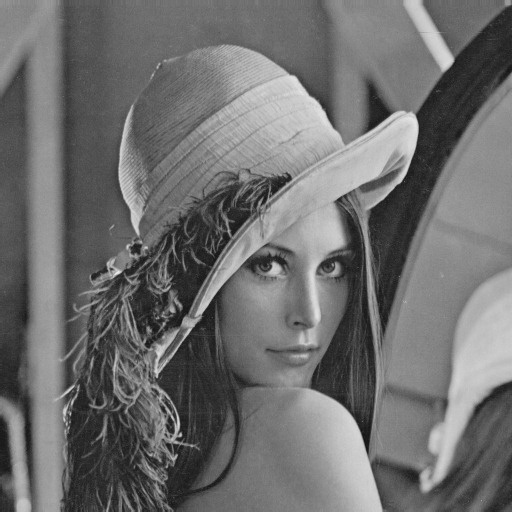
\includegraphics[width=\linewidth]{img/lena_gray.jpg}
    \caption{original}
\end{subfigure} \hspace{0.5cm}
\begin{subfigure}[b]{0.2\linewidth}
    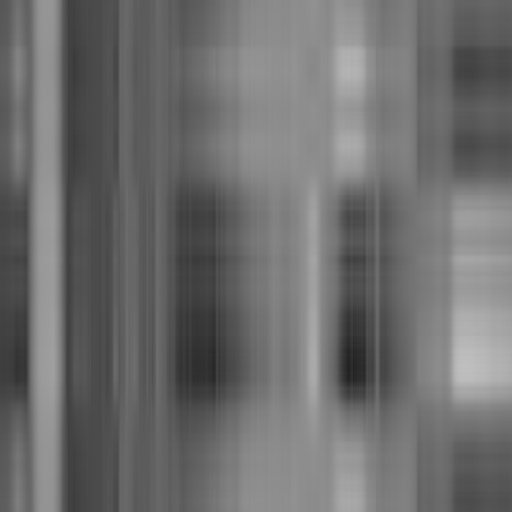
\includegraphics[width=\linewidth]{img/lena_20.jpg}
    \caption{$E(k) = 0.23$}
\end{subfigure}\\
\begin{subfigure}[b]{0.2\linewidth}
    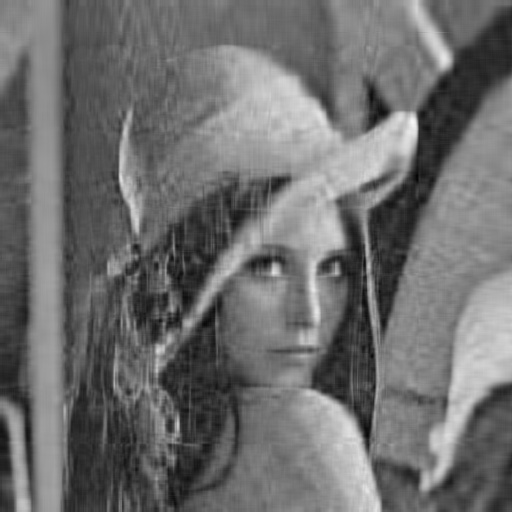
\includegraphics[width=\linewidth]{img/lena_90.jpg}
    \caption{$E(k) = 0.90$}
\end{subfigure} \hspace{0.5cm}
\begin{subfigure}[b]{0.2\linewidth}
    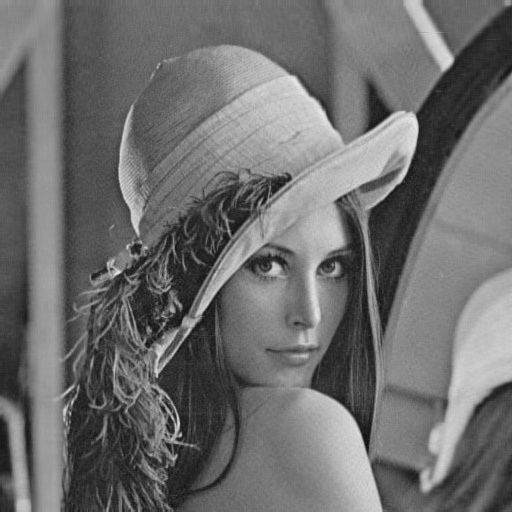
\includegraphics[width=\linewidth]{img/lena_99.jpg}
    \caption{$E(k) = 0.99$}
\end{subfigure}
\caption{A imagem \texttt{lena\_gray.jpg} em diferentes qualidades.}
\end{figure}
\FloatBarrier

Como podemos ver, a técnica apresentada torna-se extremamente eficaz na compressão de imagens, sem efetuar cálculos aritméticos enormes e inversões de matrizes. Vale lembrar do experimento ``à parte'' que fizemos no final da seção anterior. O resultado alcançado fora:
\begin{figure}[h!]
    \centering
    
\includegraphics[width=0.4\linewidth]{img/lena_E20_ultimosVS}
    \caption{Resultado do segundo experimento.}
\end{figure}

Como observado, a imagem gerada não parece nada com a imagem original, o que nos leva a concluir que as informações tomadas para gerar esse resultado não têm grande relevância, pois formam apenas um aparente borrão preto. Se olhar mais de perto, será possível observar muito discretamente as formas do rosto de Lena, como o de uma pessoa em uma noite sem lua nem estrelas.
%%%%%%%%%%%%%%%%%%%%%%%%%%%%%%
%%% referencias bibliograficas
\bibliographystyle{apalike}
% \bibliographystyle{abnt-alf}
\bibliography{biblio}

\end{document}
